\documentclass[landscape,10pt]{article}
\usepackage[latin1]{inputenc}

\usepackage{ae}
\usepackage{amssymb}
\usepackage{url}
\usepackage{xspace}

\usepackage{tikz}
\usetikzlibrary{mindmap,trees}
\usetikzlibrary{shapes}

% set up externalization
\usetikzlibrary{external}
\tikzset{external/system call={latex \tikzexternalcheckshellescape -halt-on-error
-interaction=batchmode -jobname "\image" "\texsource";
dvips -o "\image".ps "\image".dvi;
ps2eps "\image.ps"}}
\tikzexternalize

%% https://www.bu.edu/math/files/2013/08/tikzpgfmanual.pdf

\begin{document}

\tikzstyle{root concept}+=[concept color=red!60]
%% \tikzstyle{level 1 concept}+=[set style={{every child}=[concept color=orange!50]}]
%% \tikzstyle{level 2 concept}+=[set style={{every child}=[concept color=blue!20]}]


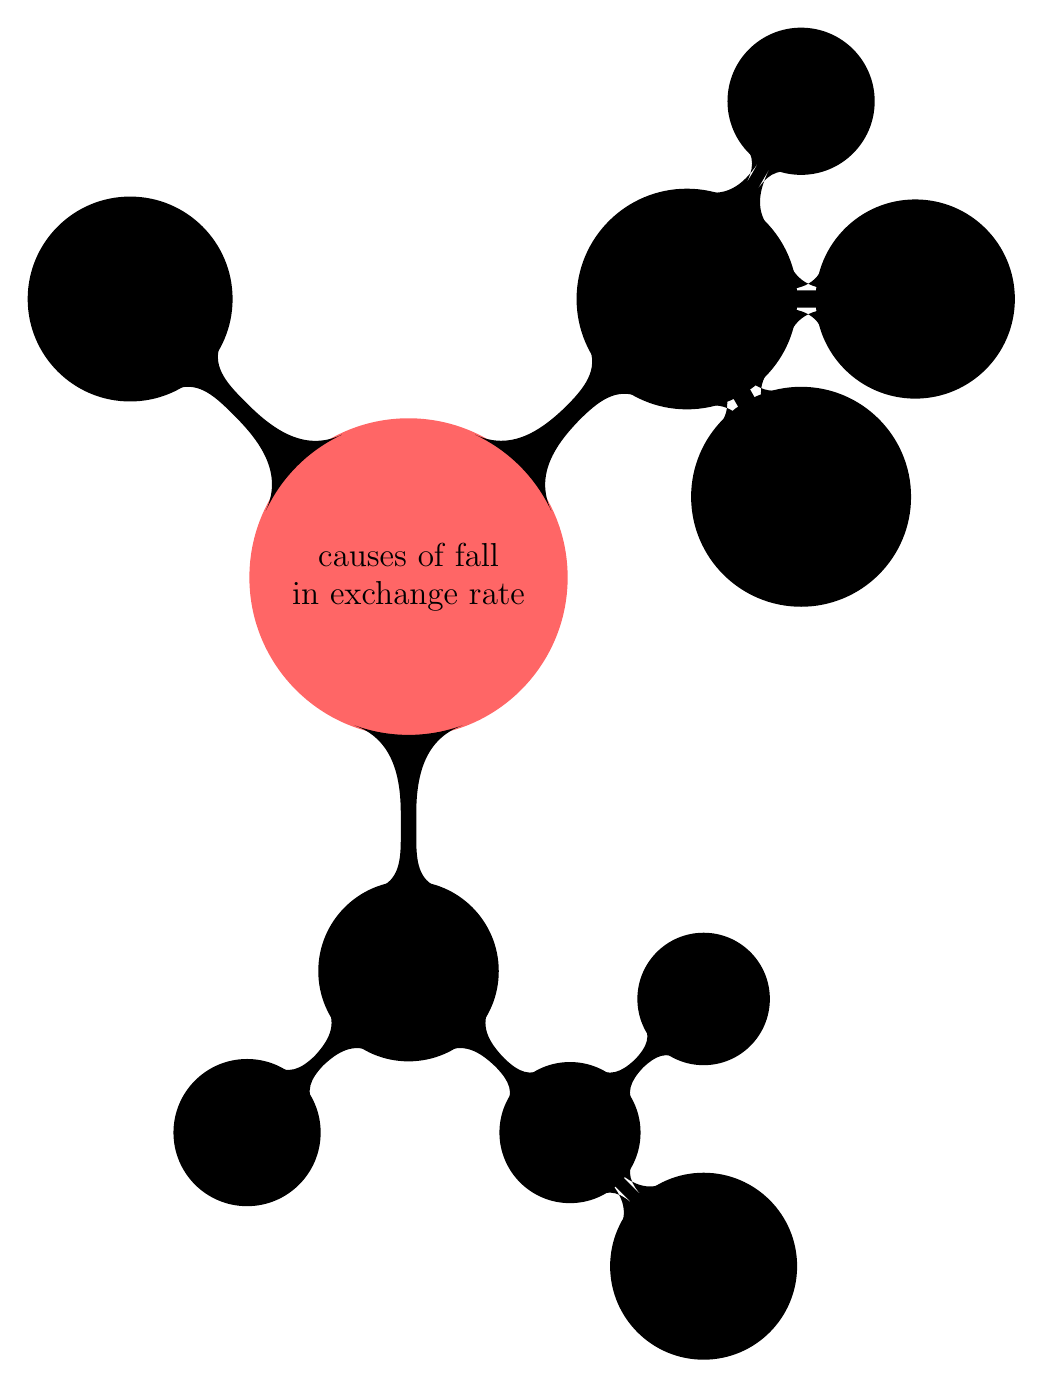
\begin{tikzpicture}[mindmap, level distance=30mm]
%%% 8-mark question %%%

      \node[concept, concept color=red!60] { causes of fall \\ in exchange rate }
      %%
      child[grow=45] 
      {
        node[concept] { \textbf{definition}: price of \\  one currency in terms of another }
        child[grow=60]  {node [concept] { \textbf{free float}: market forces } }
        child[grow=0]  {node [concept] { \textbf{fixed exchange rate}: government \\ or central bank } }
        child[grow=-60]  {node [concept] { \textbf{managed float}: influenced by \\ governmentor central bank } }
      }
      %% 
      child[grow=-90]
      {
        node[concept] { \textbf{floating exchange rate} }
        child[grow=-45]  {node [concept] { 
          \textbf{inflation} }
          child[grow=45]  {node [concept] {  imports rise \\ supply for currency rises  } } 
          child[grow=-45]  {node [concept] {  exports fall \\ (if demand is elastic) \\ demand for currency falls  } } 
          }
        child[grow=225]  {node [concept] { \textbf{lower interest rate} } }
      }
      child[grow=135] 
      {
        node[concept] { 
          \textbf{fixed exchange rate} \\ or \\ \textbf{managed float} 
          }
      }
      ;


\end{tikzpicture}

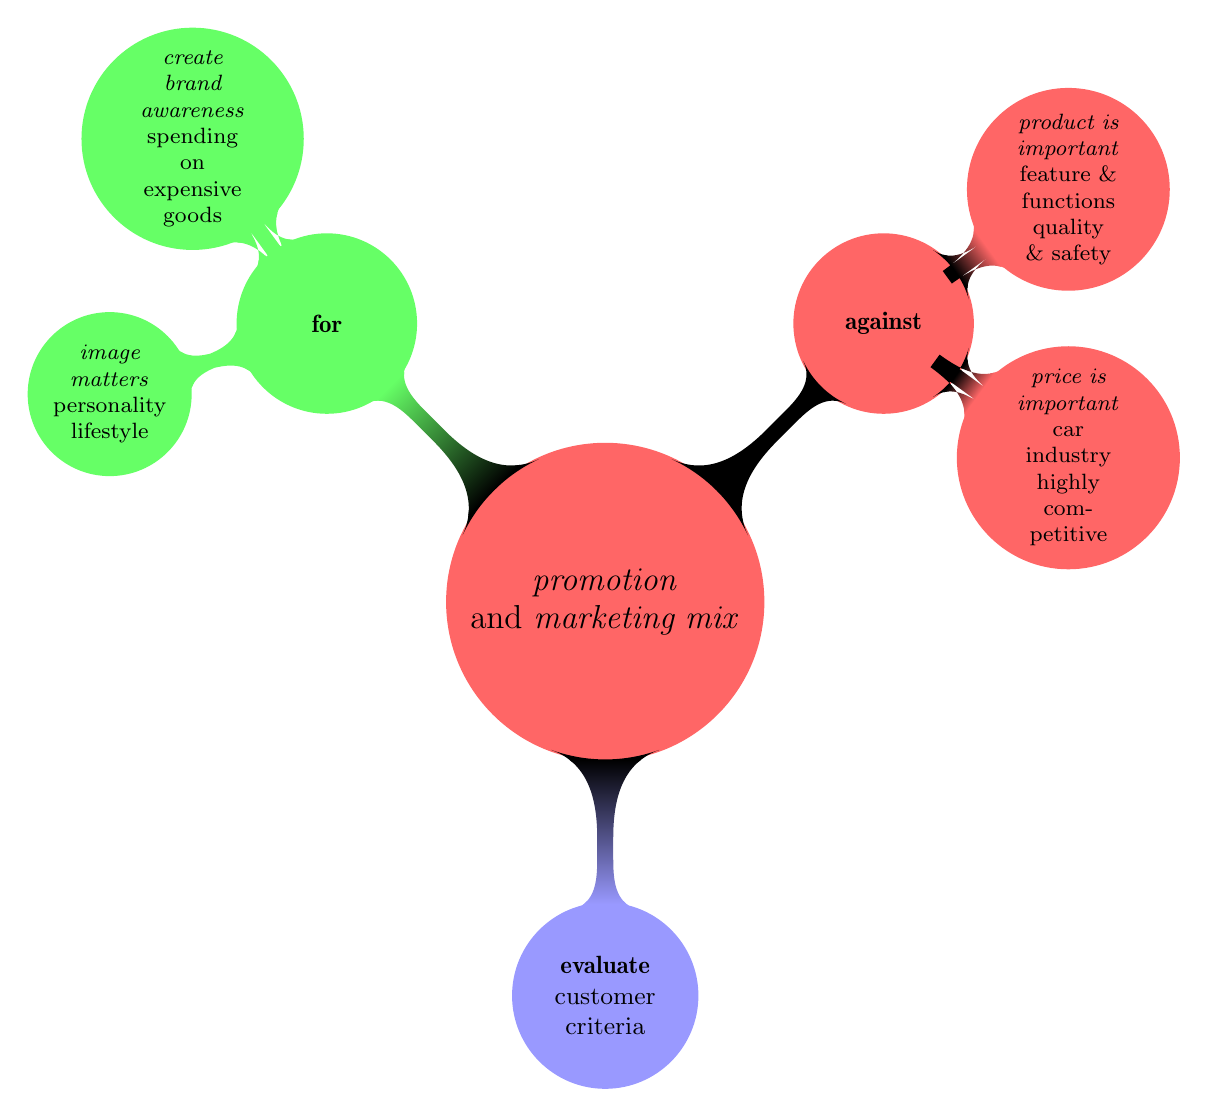
\begin{tikzpicture}[mindmap, level distance=30mm]
%%% 12-mark question %%%

      \node[concept, concept color=red!60] {\emph{promotion}\\ and \emph{marketing mix} }
      %%
      child[grow=45] 
      {
        %
        node[concept, concept color=red!60] {\textbf{against} }
        %
        child[grow=36, concept color=red!60]  {node [concept] {\emph{product is important} \\ feature \& functions \\ quality \& safety }}
        %
        child[grow=-36, concept color=red!60]  {node [concept] {\emph{price is important} \\ car industry \\ highly competitive }}
      }
      %% 
      child[grow=135, concept color=green!60]
      {
        node[concept, concept color=green!60] {\textbf{for}}
        %
        child[grow=126, concept color=green!60]  {node [concept, concept color=green!60] {\emph{create brand awareness} \\ spending on expensive goods }}
        %
        child[grow=198, concept color=green!60]  {node [concept] {\emph{image matters} \\ personality \\ lifestyle }} 
      }
      child[grow=-90, concept color=blue!40] 
      {
        node[concept, concept color=blue!40] {\textbf{evaluate} \\ customer criteria}
      }
      ;


\end{tikzpicture}



\end{document}
